\input{preamble.sty}

\lhead{АиСД, задача 2.9}
\lfoot{Михайлов Максим}
\cfoot{}
\rfoot{M3237}

\begin{document}

\section*{Условие}

Приведите контрпример для следующего алгоритма поиска размера максимального паросочетания в произвольном графе. Создать двудольный граф из \(2|V|\) вершин, для \(v\in V\) создать по вершине в обеих долях: \(l_v\) и \(r_v\).
Для каждого ребра \(vu\) создать ребра \(l_v r_u\) и \(l_u r_v\). Посчитать максимальное паросочетание в двудольном графе \(M\), в ответ выдать \(\left\lfloor \frac{|M|}{2} \right\rfloor\)

\section*{Решение}

Несложно заметить, что в двудольном графе, соответствующем \(K_3\), максимальное паросочетание имеет размер \(3\). \(\left\lfloor \frac{3}{2} \right\rfloor = 1\), поэтому для \(K_3\) алгоритм верный. Но для двух \textit{(не связанных)} \(K_3\) в двудольном графе максимальное паросочетание имеет размер \(6\) и ответ уже неверный:

\begin{figure}[h]
    \begin{minipage}[c]{0.35\textwidth}
        \centering
        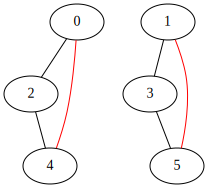
\includegraphics[width=\textwidth]{images/triangles.pdf}
    \end{minipage}\hfill
    \begin{minipage}[c]{0.65\textwidth}
        \centering
        \includegraphics[width=\textwidth]{images/triangles_conv.pdf}
    \end{minipage}\hfill
    \caption{Два \(K_3\) \textit{(слева)}, соответствующий им двудольный граф \textit{(справа)} и их паросочетания \textit{(красным)}}
\end{figure}

Если заставить алгоритм работать на отдельных КС, то он тоже не работает на следующем \textit{(найденном брутфорсом)} примере \textit{(двудольный граф на следующей странице)}:

\begin{figure}[h]
    \centering
    \includegraphics[width=\textwidth]{images/big.pdf}
\end{figure}

\begin{figure}[h]
    \centering
    \includegraphics[width=\textwidth]{images/big_conv.pdf}
    \caption{Двудольный кот, наклонивший голову влево \textit{(сверху ушки, по сторонам --- усы)}.}
\end{figure}

% \begin{minipage}[c]{0.5\textwidth}
%     \centering
%     \includegraphics[width=\textwidth]{images/big.pdf}
% \end{minipage}\hfill
% \begin{minipage}[c]{0.5\textwidth}
%     \centering
%     \includegraphics[width=\textwidth]{images/big_conv.pdf}
% \end{minipage}\hfill

\end{document}